% Inscribed regular 4-, 8- and 16-gons in the unit circle (Viete). Generated by a short script.
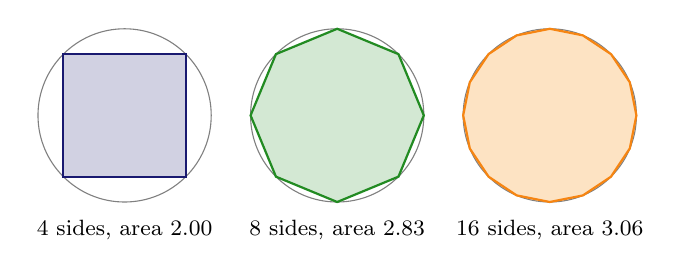
\begin{tikzpicture}[every node/.style={font=\footnotesize}]
\draw[gray] (0.0,0) circle (1.1);
\filldraw[MidnightBlue,fill=MidnightBlue!20,thick] (0.778,0.778)--(-0.778,0.778)--(-0.778,-0.778)--(0.778,-0.778)--cycle;
\node at (0.0,-1.45) {$4$ sides, area $2.00$};
\draw[gray] (2.7,0) circle (1.1);
\filldraw[ForestGreen,fill=ForestGreen!20,thick] (3.478,0.778)--(2.700,1.100)--(1.922,0.778)--(1.600,0.000)--(1.922,-0.778)--(2.700,-1.100)--(3.478,-0.778)--(3.800,-0.000)--cycle;
\node at (2.7,-1.45) {$8$ sides, area $2.83$};
\draw[gray] (5.4,0) circle (1.1);
\filldraw[BurntOrange,fill=BurntOrange!20,thick] (6.178,0.778)--(5.821,1.016)--(5.400,1.100)--(4.979,1.016)--(4.622,0.778)--(4.384,0.421)--(4.300,0.000)--(4.384,-0.421)--(4.622,-0.778)--(4.979,-1.016)--(5.400,-1.100)--(5.821,-1.016)--(6.178,-0.778)--(6.416,-0.421)--(6.500,-0.000)--(6.416,0.421)--cycle;
\node at (5.4,-1.45) {$16$ sides, area $3.06$};
\end{tikzpicture}
